
%Intro
To evaluate \FiveStars, we conducted experiments in which we used it
to solve a variety of verification tasks for a range of topologies,
configurations, and heuristic settings. The main goals of our
evaluation are to determine:
\begin{itemize}
\item What advantage is gained by discovering relevant portions of the product
automaton on-the-fly instead of pre-computing it?
\item What advantage can be gained by running \FiveStars in particular modes for
      certain \emph{types} of queries?
\item How much does the path-pruning optimization contribute to the performance of the tool?      
\item How well each mode scales with the size of topology?
\end{itemize}

%Benchmarks
We conducted our experiments using topologies drawn from
the \emph{The Internet Topology Zoo} \citep{topologyzoo} dataset, as
well as FatTree topologies, which are widely used in data centers. We
generated destination-based routing using a simple all-pairs shortest
path scheme that connects every pair of routers to each other. In the
case of the FatTree topologies, we also generated destination-based
routing between all routers on the lowest level of the tree.  Finally,
we modeled isolated slices by generating two destination-based
all-pair shortest path routing configurations, each covering
approximately half of the hosts.

We ran each algorithm and optimization over reachability,
unreachability and slicing queries on a MacBook Pro 16-inch 2023 with
an Apple M2 Max CPU and 32 GB of memory.

In the remainder of this section, we present four case studies
excerpted from the results to illustrate our answers the previously
stated questions. Complete tables of results are included
in \Cref{fig:eval-results}.

In tables and graphs, \emph{Fwd}, \emph{WP} and \emph{WPPP} correspond to on-the-fly versions of forward, weakest-precondition and weakest-precondition with path-pruning. \emph{A-Fwd}, \emph{A-Bwd} and \emph{A-WP} correspond to automata-compiled versions of forward, backward and weakest-precondition, and include compilation time. \emph{A-Comp} corresponds to automata compilation time only.

% Q1: On the fly vs automata compilation
\paragraph{What advantage is gained by pre-computing the product automata compared to
discovering relevant portions on-the-fly?}

To answer this question, we ran all our bisimulation algorithm over a slicing query over the same topology, and profiled separately the time taken in
automata compilation. As shown in Figure~\ref{fig:graph-Q1}, the
bisimulation over the compiled product automaton run faster, as they
can take advantage of dense data representations. This advantage is pronounced enough that it results in faster total time than on-the-fly discovery, even when accounting for the compilation time (in black), in all but reachability queries. For reachability queries, where the source information can be used to avoid considering large parts of the network and policy and computing irrelevant derivates, the total time is lower with on-the-fly discovery.




\begin{figure}[ht]
\begin{center}
\includegraphics[scale=0.5]{figures/rq1.png}
\end{center}
\caption{Compilation and Bisimulation time for queries over Arpanet.}
\label{fig:graph-Q1}
\end{figure}





% Q2: Different mode (forward, backward, WP and WPPP) and different query (reach, unreach, slicing)
\paragraph{What advantage can be gained by running \FiveStars in particular modes for
      certain \emph{types} of queries?}

To answer this question, we ran reachability, unreachability and
slicing queries over the same topology with all our bisimulation
algorithms.  We have plotted the results in
Figure~\ref{fig:graph-Q2}.  The forward algorithm shines on reachability
queries, where it can use the source information to only explore
portions of the product automaton relevant to the query, and it is
sufficient to prove reachability on a single connected state.  The
backward algorithm works best on unreachability queries, where query
can be answered using the unreachability over all subsequent states.
The weakest-precondition algorithm handles unreachability queries
similarly to the backward algorithms, while being the fastest by far
on slicing queries. With the path-pruning and short-circuiting
optimization on, the weakest-precondition algorithm also performs
faster than the forward algorithm on reachability queries. However,
these optimizations result in a slowdown on unreachability and slicing
queries.


\begin{figure}
\begin{center}
\includegraphics[scale=0.5]{figures/rq2.png}
\end{center}
\caption{Total time for all algorithms on different queries}
\label{fig:graph-Q2}
\end{figure}


%
\begin{comment}
\begin{figure}[ht]
\begin{center}
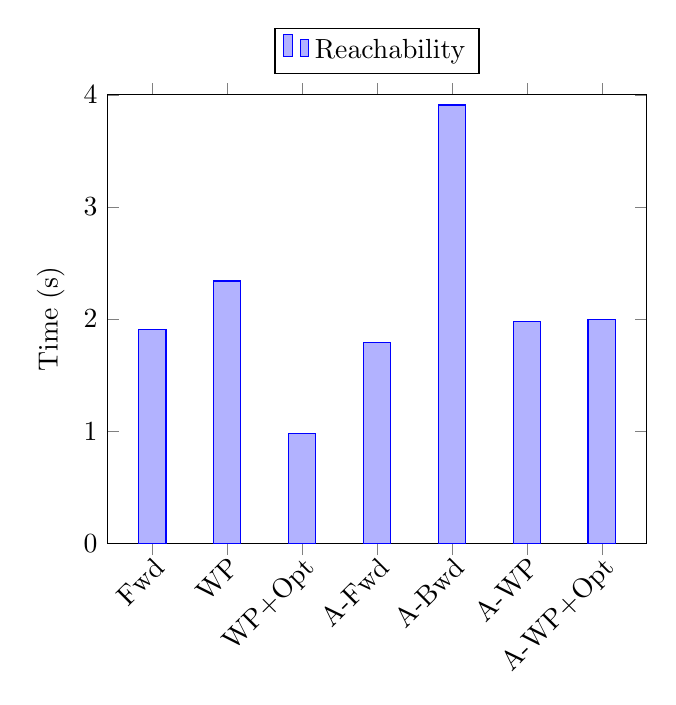
\begin{tikzpicture}
\begin{axis}[
        ybar,
	ylabel= Time (s),
        symbolic x coords= {Fwd, WP, WP+Opt, A-Fwd, A-Bwd, A-WP, A-WP+Opt},
        xtick = {Fwd, WP, WP+Opt, A-Fwd, A-Bwd, A-WP, A-WP+Opt},
        x tick label style={rotate=45, anchor=north east, inner sep=0mm},        
        ymin=0,
        ymax=4,
        legend style={at={(0.5,1.15)},        
	anchor=north,legend columns=-1},
]
% Reachability
\addplot
	coordinates { (Fwd, 1.91) (WP, 2.34) (WP+Opt, 0.98) (A-Fwd, 1.79) (A-Bwd, 3.91) (A-WP, 1.98) (A-WP+Opt, 2.00)};


\legend{Reachability}
\end{axis}
\end{tikzpicture}
\end{center}
\caption{Total time for reachability queries over Sanet}
\label{fig:graph-Q21}
\end{figure}

\begin{figure}[ht]
\begin{center}
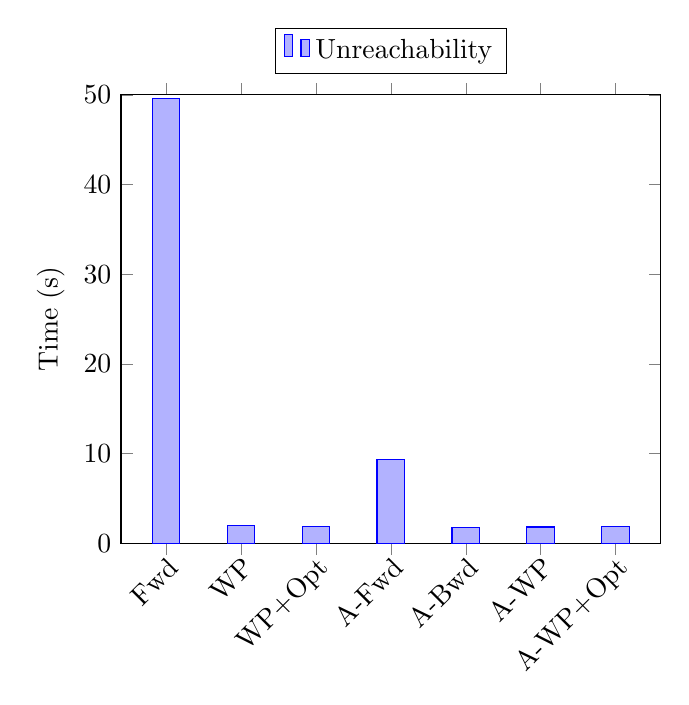
\begin{tikzpicture}
\begin{axis}[
        ybar,
	ylabel= Time (s),
        symbolic x coords= {Fwd, WP, WP+Opt, A-Fwd, A-Bwd, A-WP, A-WP+Opt},
        xtick = {Fwd, WP, WP+Opt, A-Fwd, A-Bwd, A-WP, A-WP+Opt},
        x tick label style={rotate=45, anchor=north east, inner sep=0mm},        
        ymin=0,
        ymax=50,
        legend style={at={(0.5,1.15)},        
	anchor=north,legend columns=-1},
]
% Unreachability
\addplot
	coordinates { (Fwd, 49.61) (WP, 1.98) (WP+Opt, 1.85) (A-Fwd, 9.36) (A-Bwd, 1.79) (A-WP, 1.81) (A-WP+Opt, 1.82)};
\legend{Unreachability}
\end{axis}
\end{tikzpicture}
\end{center}
\caption{Total time for unreachability queries over Sanet}
\label{fig:graph-Q22}
\end{figure}

\begin{figure}[ht]
\begin{center}
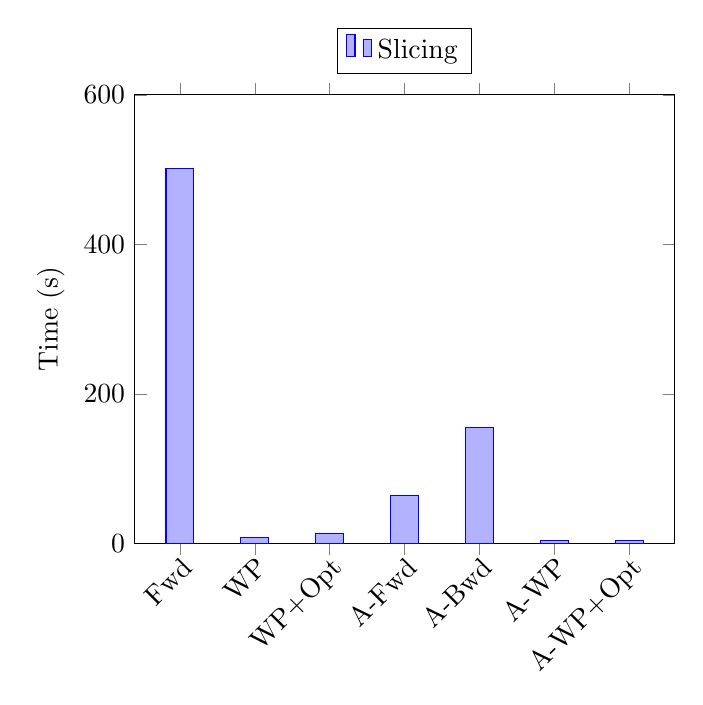
\begin{tikzpicture}
\begin{axis}[
        ybar,
	ylabel= Time (s),
        symbolic x coords= {Fwd, WP, WP+Opt, A-Fwd, A-Bwd, A-WP, A-WP+Opt},
        xtick = {Fwd, WP, WP+Opt, A-Fwd, A-Bwd, A-WP, A-WP+Opt},
        x tick label style={rotate=45, anchor=north east, inner sep=0mm},        
        ymin=0,
        ymax=600,
        legend style={at={(0.5,1.15)},        
	anchor=north,legend columns=-1},
]
% Slicing
\addplot
	coordinates { (Fwd, 501.94) (WP, 7.36) (WP+Opt, 13.19) (A-Fwd, 63.35) (A-Bwd, 155.44) (A-WP, 3.59) (A-WP+Opt, 3.60)};

\legend{Slicing}
\end{axis}
\end{tikzpicture}
\end{center}
\caption{Total time for slicing queries over Sanet}
\label{fig:graph-Q23}
\end{figure}
\end{comment}


% Q3: Effect of optimization (WP/WPPP) and short circuiting
\paragraph{How much does the path-pruning optimization contribute to the performance of the tool?}

% Deltacom reachability?
To answer this question, we ran the on-the-fly bisimulation algorithm
on reachability with various optimization turned on.  We plotted the
total bisimulation time in Figure~\ref{fig:graph-Q3}.  As described in
previous sections, path pruning allows weakest-precondition algorithm
to only consider edges which are relevant to the initial query,
resulting in significantly faster processing time. The
short-circuiting optimization stops the bisimulation as soon as a path
is found between the hosts -- in general, this results in time saved
proportional to how close the source and the destination are.

\begin{figure}[ht]
\begin{center}
\begin{comment}
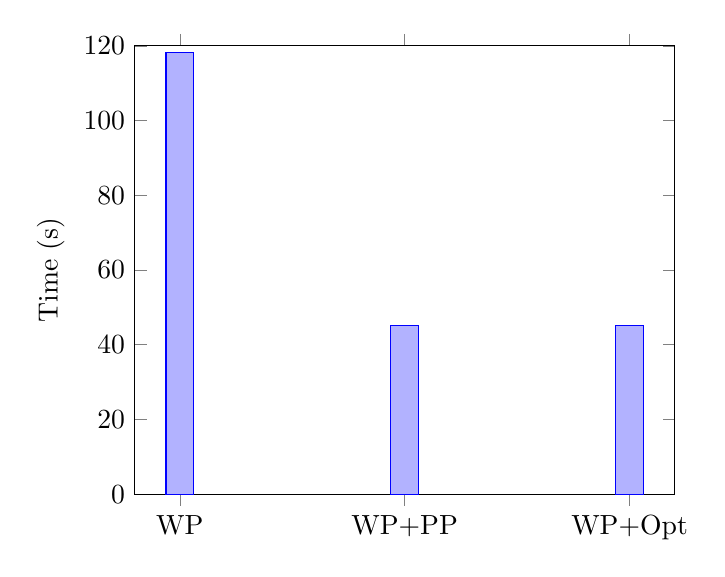
\begin{tikzpicture}
\begin{axis}[
        ybar,
	ylabel=Time (s),
        symbolic x coords= {WP, WP+PP, WP+Opt},
        xtick = {WP, WP+PP, WP+Opt},
        ymin=0,
        ymax=120
]
\addplot coordinates { (WP,118.13) (WP+PP,45.23) (WP+Opt,45.20)};
\end{axis}
\end{tikzpicture}
\end{comment}
\includegraphics[scale=0.5]{figures/rq3.png}
\end{center}
\caption{Total time for reachability query over TopologyZoo topologies}
\label{fig:graph-Q3}
\end{figure}

% Q4: How well do each mode scaled for slicing
\paragraph{How well each mode scales with the size of topology?}

We ran each of our bisimulation algorithm over real topologies from TopologyZoo
in order to evaluate how they scale with topologies of different sizes, and plotted the results in
Figure~\ref{fig:graph-Q4}. We have also experimented with using number of nodes and number of edges instead of size of the routing policy, but found the latter a better predictor of complexity for queries. These tests show how the weakest-precondition algorithm
scales much better than forward bisimulation. As discussed earlier,
for slicing query, the extra computation introduced by the
path-pruning and short-circuiting optimization ends up slowing down
the bisimulation compared to the same algorithm without optimization whenever the solver cannot make use of information in the query to prune significant portion of the bisimulation, and as such should be reserved to, for example, reachability queries.

\begin{figure}[ht]
\begin{center}
\begin{comment}
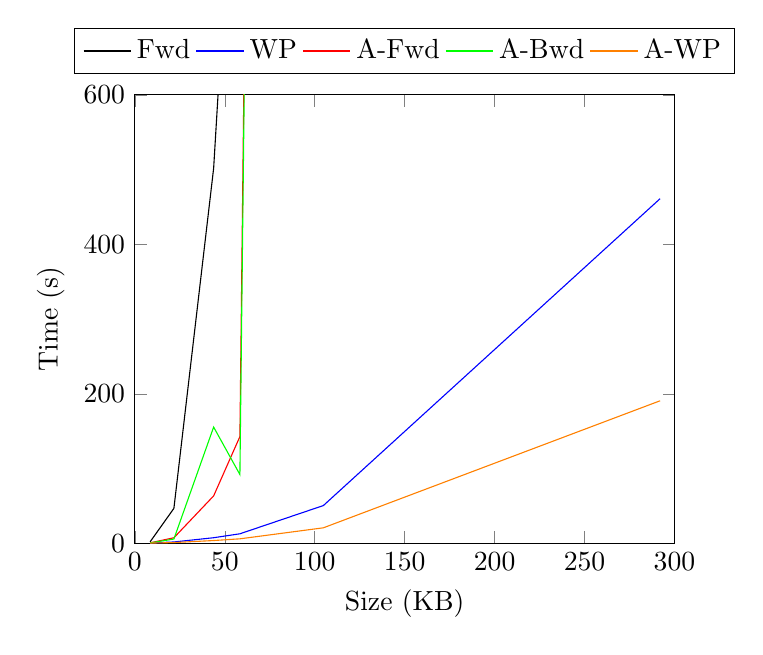
\begin{tikzpicture}
\begin{axis}[
        xlabel=Size (KB),
	ylabel=Time (s),
        xmin=0,
        xmax= 300,
        ymin=0,
        ymax=600,
        legend style={at={(0.5,1.15)},        
	anchor=north,legend columns=-1},        
]
% forward
\addplot [color=black]
	coordinates { (8.5, 1.92) (21.7, 46.63) (43.8, 501.94) (58.4, 1088.79) (104.8, 10000) (292, 10000) };

% wp
\addplot [color=blue]
	coordinates { (8.5, 0.27) (21.7, 1.68) (43.8, 7.36) (58.4, 12.62) (104.8, 50.42) (292, 461.14) };

% a-fwd
\addplot [color=red]
	coordinates { (8.5, 0.57) (21.7, 7.31) (43.8, 63.35) (58.4, 142.75) (104.8, 10000) (292, 10000) };

% a-bwd
\addplot [color=green]
	coordinates { (8.5, 0.40) (21.7, 5.61) (43.8, 155.44) (58.4, 91.90) (104.8, 10000) (292, 10000) };

% a-wp
\addplot [color=orange]
	coordinates { (8.5, 0.18) (21.7, 0.89) (43.8, 3.59) (58.4, 5.88) (104.8, 20.62) (292, 190.65) };


\legend{Fwd,WP, A-Fwd, A-Bwd, A-WP}

\end{axis}
\end{tikzpicture}
\end{comment}
\includegraphics[scale=0.5]{figures/rq4.png}
\end{center}
\caption{Total time for slicing queries over TopologyZoo topologies}
\label{fig:graph-Q4}
\end{figure}


% Something about Stanford
We have also experimented with running queries over the Stanford
backbone network (sourced from \cite{hsa}), which has a sizeable
(around 20 MB) IP-based routing policy. In order to make this routing
policy more tractable, we used static-field specializations, a
technique described in Libra \citep{libra}, which specialize the
routing of the network according to fields of packets that do not
change during routing, so that we can answer queries about the whole
network by solving multiple, smaller queries about each way it could
be specialized. In the case of the Stanford backbone network, the IP
destination fields do not change, and specializing it results in
$2348$ subnets. Queries can be run in parallel on each of the subnets,
taking on average $0.2$ seconds for reachability and $0.3$ seconds for
unreachability queries.

